\documentclass[11pt,wide]{article}

\usepackage{polski}
\usepackage[utf8]{inputenc}

\usepackage{graphicx} 

\usepackage{mathtools}
\usepackage{amsthm}
\usepackage{verbatim}
\usepackage{xcolor}

\usepackage{hyperref}


\hypersetup{
    colorlinks=true,
    linkcolor=blue,
    filecolor=magenta,      
    urlcolor=cyan,
    citecolor=green,
    pdftitle={Sharelatex Example},
    bookmarks=true,
}

\newcommand\numeq[1]%
  {\stackrel{\scriptscriptstyle \mkern-1.5mu#1\mkern-1.5mu }{=}}

\newtheorem{thm}{Twierdzenie}
\newtheorem{remark}{Uwaga}
\newtheorem{lemat}{Lemat}
\newtheorem{wniosek}{Wniosek}
\newtheorem{definicja}{Definicja}
\newtheorem{ciekawostka}{Ciekawostka}
\newtheorem{przyklad}{Przykład}
\newtheorem{rysunek}{Rysunek}

% Marginesy
\topmargin=-0.45in
\evensidemargin=0in
\oddsidemargin=0in
\textwidth=6.5in
\textheight=9.0in
\headsep=0.25in

\title{Analiza numeryczna (M) - Pracownia 2 \\ Zadanie P2.17\\
Kwadratury Newtona-Cotesa i metoda Romberga}
\date{Wrocław, Grudzień 14, 2019}
\author{Jakub Kuciński, prowadzący Witold Karczewski}

\begin{document}

\maketitle
\thispagestyle{empty} 
\tableofcontents


\section{Wprowadzenie}
Całkowanie funkcji jest bardzo trudnym zadaniem. Dla wielu funkcji ciężko wyprowadzić jawny wzór funkcji pierwotnej, a dla niektórych takowe nawet nie istnieją. W wielu przypadkach wystarczające jest jednak poznanie tylko przybliżonej wartości szukanej całki oznaczonej. Dla takich problemów bardzo skutecznym rozwiązaniem jest całkowanie numeryczne. W sprawozdaniu omówione zostaną kwadratury proste i złożone Newtona-Cotesa niższych rzędów oraz metoda Romberga, będące jednymi z podstawowych metod całkowania numerycznego. Sprawdzona zostanie również ich dokładność dla całek oznaczonych z wielomianów, funkcji wymiernych oraz funkcji wymiernych dwóch zmiennych sin(x) i cos(x).
\pagebreak

\section{Metody Newtona-Cotesa}
Metody Newtona-Cotesa są to metody całkowania numerycznego polegające na przybliżaniu wartości całki z funkcji przez całkę z wielomianu interpolacyjnego Lagrange'a dla równo oddalonych punktów węzłowych, takich że \(a = x_0 < x_1 < \ldots < x_n  = b\).
Mamy więc
\begin{equation}
\int_a^b f(x)\mathop{dx} \approx \int_a^b L_n(x) \mathop{dx} = \int_a^b \sum_{i=0}^n f(x_i) \lambda_i \mathop{dx} = \sum_{i=0}^n f(x_i) \int_a^b  \lambda_i \mathop{dx}
\end{equation}
gdzie \(\lambda_i \) wyraża się wzorem
\begin{equation}
\lambda_i = \prod_{\substack{j=0 \\ j \neq i}}^n \frac{x-x_j}{x_i-x_j}
\end{equation}
Ustalając \(\displaystyle h =\frac{b - a}{n}\) czyli odległość dwóch sąsiednich punktów węzłowych oraz przyjmując t, takie że \(x = a + t\cdot h\) otrzymujemy
\begin{equation}
\int_a^b \lambda_i = \int_a^b \prod_{\substack{j=0 \\ j \neq i}}^n \frac{x-x_j}{x_i-x_j} \mathop{dx} = h \int_0^n \prod_{\substack{j=0 \\ j \neq i}}^n \frac{t-j}{i-j} \mathop{dt}
\end{equation}
Oznaczając współczynniki kwadratury Newtona-Cotesa \(\displaystyle A_i = h \int_0^n \prod_{\substack{j=0 \\ j \neq i}}^n \frac{t-j}{i-j} \mathop{dt}\) dostajemy
\begin{equation}
\int_a^b f(x)\mathop{dx} \approx \sum_{i=0}^n f(x_i) A_i
\end{equation}
\\
Można udowodnić następujące twierdzenie:
\begin{thm}
\label{tw:WspKwNewCot}
\(A_i = A_{n-i} \)
\end{thm}
\begin{proof}
\begin{equation}
A_i = h \int_0^n \prod_{\substack{j=0 \\ j \neq i}}^n \frac{t-j}{i-j} \mathop{dt} = h (-1)^{n-i} \frac{1}{i!(n-i)!} \int_0^n \prod_{\substack{j=0 \\ j \neq i}}^n (t-j) \mathop{dt}
\end{equation}
Wykonajmy podstawienie \(t = n - u, \ \mathop{dt} = - \mathop{du}\)
\begin{equation}
A_i = h (-1)^{n-i} \frac{1}{i!(n-i)!} \int_n^0 -\prod_{\substack{j=0 \\ j \neq i}}^n (n-u-j) \mathop{dt} = h (-1)^{n-i} \frac{1}{i!(n-i)!} \int_0^n (-1)^n \prod_{\substack{j=0 \\ j \neq i}}^n (u-(n-j)) \mathop{dt}
\end{equation}
Zauważmy, że
\begin{equation}
\prod_{\substack{j=0 \\ j \neq i}}^n (u-(n-j)) \mathop{dt} = \prod_{\substack{j=0 \\ j \neq n-i}}^n (u-j) \mathop{dt}
\end{equation}
Stąd
\begin{equation}
A_i = h (-1)^{n-i} (-1)^{-n}  \frac{1}{i!(n-i)!} \int_0^n \prod_{\substack{j=0 \\ j \neq n-i}}^n (u-j) \mathop{dt} = h (-1)^{i}  \frac{1}{i!(n-i)!} \int_0^n \prod_{\substack{j=0 \\ j \neq n-i}}^n (u-j) \mathop{dt} = A_{n-i}
\end{equation}
\end{proof}


\subsection{Metoda trapezów}
Metoda trapezów to metoda Newtona-Cotesa zastosowana dla wielomianu interpolacyjnego Lagrange'a pierwszego stopnia, czyli dla \(n = 1\).  W celu wyliczenia jawnego wzoru trapezów wyliczmy \(A_0\) i \(A_1\):
\begin{equation}
A_0 = h \int_0^1 \frac{t-1}{0-1} \mathop{dt} = -h \int_0^1 (t-1) \mathop{dt} = -h\Big(\frac{t^2}{2} - t\Big)\Big|_{0}^{1} = \frac{h}{2}
\end{equation}
\begin{equation}
A_1 \numeq{\eqref{tw:WspKwNewCot}} A_{1-1} = A_0 = \frac{h}{2} = \frac{b - a}{2}
\end{equation}
Stąd otrzymujemy wzór trapezów:
\begin{equation} \label{wzor:WzorTrapezow}
\int_a^b f(x)\mathop{dx} \approx \sum_{i=0}^1 f(x_i) A_i = f(x_0) A_0 + f(x_1) A_1 = \frac{h}{2} (f(x_0) + f(x_1))
\end{equation}
Błąd metody trapezów wynosi
\begin{equation} \label{wzor:BladTrapezow}
R_1^T(f) = - \frac{h^3}{12}f^{(2)}(\xi) = - \frac{(b-a)^3}{12}f^{(2)}(\xi)
\end{equation}
dla pewnego \(\xi \in (a, b)\).

\subsection{Metoda Simpsona}
Metoda Simpsona to kolejna metoda Newtona-Cotesa, tym razem użyta dla wielomianu interpolacyjnego drugiego stopnia \((n = 2)\). Liczymy \(A_0\), \(A_1\) i \(A_2\):
\begin{equation}
A_0 \numeq{\eqref{tw:WspKwNewCot}} A_2 = h \int_0^2 \frac{(t-1)(t-2)}{(0-1)(0-2)} \mathop{dt} = \frac{h}{2} \int_0^2 (t^2-3t+2) \mathop{dt} = \frac{h}{2} \Big(\frac{t^3}{3} - \frac{3t^2}{2} + 2t\Big)\Big|_{0}^{2} = \frac{h}{3} = \frac{b-a}{6}
\end{equation}
\begin{equation}
A_1 = h \int_0^2 \frac{(t-0)(t-2)}{(1-0)(1-2)} \mathop{dt} = -h \int_0^2 (t^2-2t) \mathop{dt} = -h \Big(\frac{t^3}{3} - t^2\Big)\Big|_{0}^{2} = \frac{4h}{3} = \frac{4(b-a)}{6}
\end{equation}
Stąd otrzymujemy wzór Simpsona:
\begin{equation} \label{wzor:WzorSimpsona}
\int_a^b f(x)\mathop{dx} \approx \sum_{i=0}^2 f(x_i) A_i = \frac{h}{3} (f(x_0) + 4f(x_1) + f(x_2))
\end{equation}
Błąd metody Simpsona wynosi
\begin{equation} \label{wzor:BladSimpsona}
R_1^S(f) = - \frac{h^5}{90}f^{(4)}(\xi) = - \frac{(b-a)^5}{2880}f^{(4)}(\xi)
\end{equation}
dla pewnego \(\xi \in (a, b)\).

\section{Złożone kwadratury Newtona-Cotesa}
W celu polepszenia dokładności obliczania przybliżonej wartości całki można rozbić całkowany przedział na kilka podprzedziałów, na każdym z nich zastosować kwadraturę Newtona-Cotesa, a otrzymane wyniki zsumować. Takie przybliżenie wartości całki nazywamy złożoną kwadraturą Newtona-Cotesa.
\begin{equation}
\int_a^b f(x)\mathop{dx} = \sum_{i=1}^n \int_{x_{i-1}}^{x_i}  f(x) \mathop{dx} \approx \sum_{i=1}^n \int_{x_{i-1}}^{x_i} L_i(x) 
\end{equation}

\subsection{Złożona metoda trapezów}
Złożona metoda trapezów to złożona kwadratura Newtona-Cotesa, w której do przybliżania całek na poszczególnych podprzedziałach liczonej całki używamy metody trapezów. Można wyrazić ją wzorem
\begin{equation}
\int_a^b f(x)\mathop{dx} = \sum_{i=1}^n \int_{x_{i-1}}^{x_i}  f(x) \mathop{dx} \approx \sum_{i=1}^n \frac{x_i-x_{i-1}}{2}(f(x_{i-1}) +  f(x_{i})) = \frac{1}{2} \sum_{i=1}^n (x_i-x_{i-1})(f(x_{i-1}) +  f(x_{i}))
\end{equation}
Dla przedziałów równej długości mamy
\begin{equation}
\frac{1}{2} \sum_{i=1}^n (x_i-x_{i-1})(f(x_{i-1}) +  f(x_{i})) = \frac{b-a}{2n} \sum_{i=1}^n (f(x_{i-1}) + f(x_{i})) = \frac{b-a}{2n} \left((f(a) + f(b) + 2\sum_{i=1}^{n-1} f(x_{i})\right)
\end{equation}
Podstawiając \(\displaystyle x_i = a + i \frac{b-a}{n}\) dostajemy
\begin{equation} \label{wzor:WzorZlozonyTrapezow}
\int_a^b f(x)\mathop{dx} \approx \frac{b-a}{2n} \left(f(a) + f(b) + 2\sum_{i=1}^{n-1} f\left(a + i \frac{b-a}{n}\right)\right) = T_n
\end{equation}
Błąd złożonej metody trapezów wynosi
\begin{equation} \label{wzor:BladZlozonyTrapezow}
R_n^T(f) = - \frac{h^3}{12}n \cdot f^{(2)}(\xi) = - \frac{(b-a)^3}{12n^2}f^{(2)}(\xi)
\end{equation}
dla pewnego \(\xi \in (a, b)\).
\\ \\
Można również zauważyć, że zachodzi zależność 
\begin{align}\label{wzor:WzorRekurencyjnyTrapezow}
T_{2n} = \frac{b-a}{4n} \Bigg(f(a) + f(b) + 2\sum_{i=1}^{2n-1} f\bigg(a + i & \frac{b-a}{2n}\bigg)\Bigg) = \frac{T_n}{2} + \frac{b-a}{4n}  \cdot 2\sum_{i=1}^{n} f\Bigg(a + \Big(2i-1\Big) \frac{b-a}{2n}\Bigg) = \\
= \frac{T_n}{2} + \frac{b-a}{2n} \sum_{i=1}^{n} & f\Bigg(a + i \frac{b-a}{n} - \frac{b-a}{2n}\Bigg)
\end{align}
Wzór ten pozwala zoptymalizować wyliczanie kolejnych przybliżeń \(\int_a^b f(x)\mathop{dx}\) w przypadku, gdy zagęszczamy liczbę przedziałów dwukrotnie w każdej iteracji algorytmu, aż do momentu osiągnięcia wymaganej precyzji wyniku. W każdej iteracji możemy skorzystać z wyliczonego wcześniej przybliżenia i doliczyć drugą połowę wartości. Własność ta może mieć bardzo znaczący wpływ na wydajność algorytmu, jeśli obliczanie wartości funkcji jest bardzo kosztowne.

\subsection{Złożona metoda Simpsona}
Złożona metoda Simpsona to złożona kwadratura Newtona-Cotesa, w której do przybliżania całek na poszczególnych podprzedziałach liczonej całki używamy metody Simpsona. Przy założeniu, że liczba przedziałów jest parzysta, można wyrazić ją wzorem
\begin{equation}
\int_a^b f(x)\mathop{dx} \approx \frac{h}{3}\sum_{i=1}^{n/2} \Bigg(f(x_{2i-2}) + f(x_{2i-1}) + f(x_{2i})\Bigg) = \frac{h}{3}\Bigg(f(a) + f(b) + 4\sum_{i=1}^{n/2} f(x_{2i}) + 2\sum_{i=1}^{n/2 - 1} f(x_{2i-1})\Bigg)
\end{equation}
Podstawiając \(\displaystyle x_i = a + i \frac{b-a}{n}\) dostajemy
\begin{equation} \label{wzor:WzorZlozonySimpsona}
\int_a^b f(x)\mathop{dx} \approx \frac{b-a}{3n}\Bigg(f(a) + f(b) + 4\sum_{i=1}^{n/2} f\bigg(a + (2i-1) \frac{b-a}{n}\bigg) + 2\sum_{i=1}^{n/2 - 1} f\left(a + \frac{b-a}{n}\right)\Bigg)2i 
\end{equation}
Błąd złożonej metody trapezów wynosi
\begin{equation} \label{wzor:BladZlozonySimpsona}
R_n^S(f) = - \frac{h^5}{90} \cdot \frac{n}{2} \cdot f^{(4)}(\xi) = - \frac{(b-a)^5}{2880n^4}f^{(4)}(\xi)
\end{equation}
dla pewnego \(\xi \in (a, b)\).

\section{Metoda Romberga}
Metoda Romberga jest to metoda całkowania numerycznego polegająca na zmniejszaniu błędów przybliżeń całki \(\int_a^b f(x)\mathop{dx}\) policzonych przy użyciu złożonej metody trapezów w równo oddalonych punktach węzłowych wykorzystując ekstrapolacje Richardsona.
\\
\begin{thm} \label{tw:BladTrapezow}
Niech \(T_k\) oznacza wynik złożonej metody trapezów dla k podprzedziałów, I wartość  \(\int_a^b f(x)\mathop{dx}\) oraz \(h\) długość przedziałów, czyli \(\frac{b-a}{k}\). Wtedy:
\begin{equation}
T_k = I + K_1 h^2 + K_2 h^4 + K_3 h^6 + \ldots
\end{equation}
gdzie \(K_1, K_2, K_3, \ldots \) są pewnymi stałymi niezależnymi od k.
\end{thm}
Korzystając z powyższego twierdzenia dostajemy:
\begin{equation}
T_k = I + K_1 h^2 + K_2 h^4 + K_3 h^6 + \ldots
\end{equation}
oraz
\begin{equation}
T_{2k} = I + K_1 \frac{h^2}{4} + K_2 \frac{h^4}{16} + K_3 \frac{h^6}{64} + \ldots
\end{equation}
Stąd można zauważyć, że
\begin{equation}
R = \frac{4T_{2k} - T_k}{4 - 1} = I + L_1 h^4 + \ldots
\end{equation}
Zatem \(R\) jest lepszym przybliżeniem, bo błąd został zredukowany do poziomu \(\mathcal{O}(h^4)\). Metoda Romberga polega na wielokrotnym zastosowaniu tego samego spostrzeżenia dla kolejnych wartości \(T_k\) oraz już ich poprawionych przybliżeń \(R\). Można ją zapisać w postaci rekurencyjnej:
\begin{align}
& R_{0,0} = \frac{b - a}{2} (f(a) + f(b))\\
& R_{n, 0} \numeq{\eqref{wzor:WzorRekurencyjnyTrapezow}} \frac{R_{n-1, 0}}{2} + \frac{b-a}{2^n} \sum_{i=1}^{2^{n-1}}f\bigg(a+(2i-1) \frac{b-a}{2^n}\bigg) \\
& R_{n, m} = \frac{4^m R_{n, m-1} - R_{n-1, m-1}}{4^m - 1}
\end{align}
gdzie \(n \leq m\) i \(1 \leq m\). \\ 
Wyrazy \(R_{n,0}\) odpowiadają wartościom złożonej metody trapezów zastosowanej dla \(2^n\) przedziałów.\\
Można zauważyć, że wyrazy \(R_{n, 1}\) odpowiadają złożonej metodzie Simpsona.\\
Oznaczając \(h_n = \frac{b-a}{2^n}\) bład przybliżenia \(R_{n,m}\) jest klasy \(\mathcal{O}(h_n^{2m+2})\).

\pagebreak
\section{Testy numeryczne}
Dla porównania dokładności wyników wyżej omówionych metod przedstawione zostaną eksperymenty numeryczne dla wybranych całek z funkcji wielomianowych i wymiernych. Algorytmy zostały zaimplementowane w języku Julia. Wykorzystane wyniki funkcji quadgk z biblioteki QuadGK zostały uznane za dokładne w celu przybliżonego wyznaczenia błędów opisanych metod. Dla każdej z~wybranych funkcji zostaną przedstawione analogicznie dwa wykresy. Pierwszy będzie przedstawiał wykres funkcji na całkowanym przedziale, a drugi liczbę dokładnych cyfr w systemie dwójkowym wyników otrzymanych za pomocą metod trapezów, Simpsona oraz Romberga. Oś OX odpowiada liczbie podprzedziałów całkowania w skali wykładniczej, tzn. liczba k na osi oznacza \(2^k\) podprzedziałów. 

\subsection{Całka z wielomianu}
Pierwszy eksperyment został przeprowadzony na \(\displaystyle \int_{-2}^{10} (7x -1)\mathop{dx} \)
\begin{figure}[h!]
	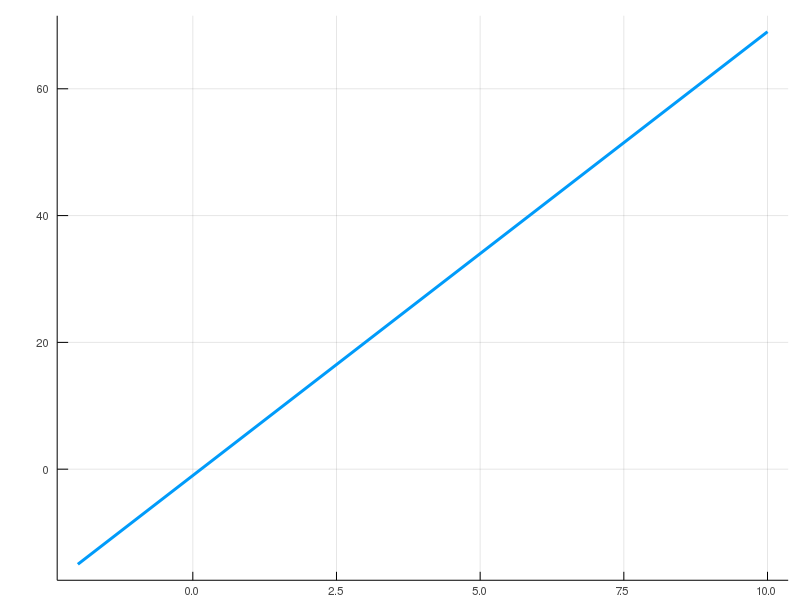
\includegraphics[width=70mm,scale=0.5]{wiel1}
	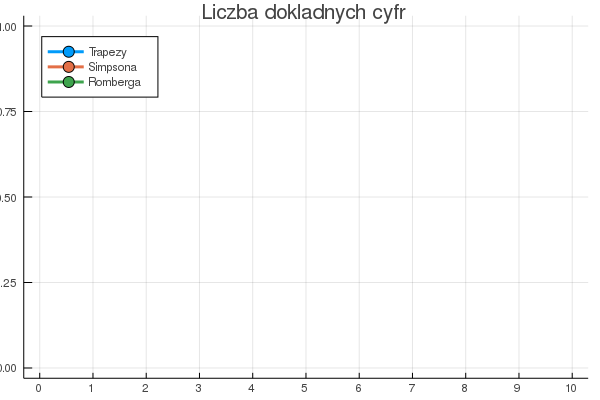
\includegraphics[width=80mm,scale=0.5]{wiel_blad1}
\end{figure}
\begin{remark}
\centering
Wykres funkcji \(f(x) = 7x -1 \) oraz liczba dokładnych cyfr wyników.
\end{remark}
Widać, że wszystkie wyniki dla omawianych metod są dokładne. Jest to naturalne, skoro metoda trapezu jest rzędu 1, a metoda Simpsona rzędu 3. Metoda Romberga opiera się na metodzie trapezów, więc skoro metoda trapezów była dokładna, to metoda Romberga również. 
\pagebreak

Kolejny eksperyment przeprowadzono na \(\displaystyle \int_{-4}^{4} (6x^3 + 21x^2 - 138x + 63)\mathop{dx} \)
\begin{figure}[h!]
	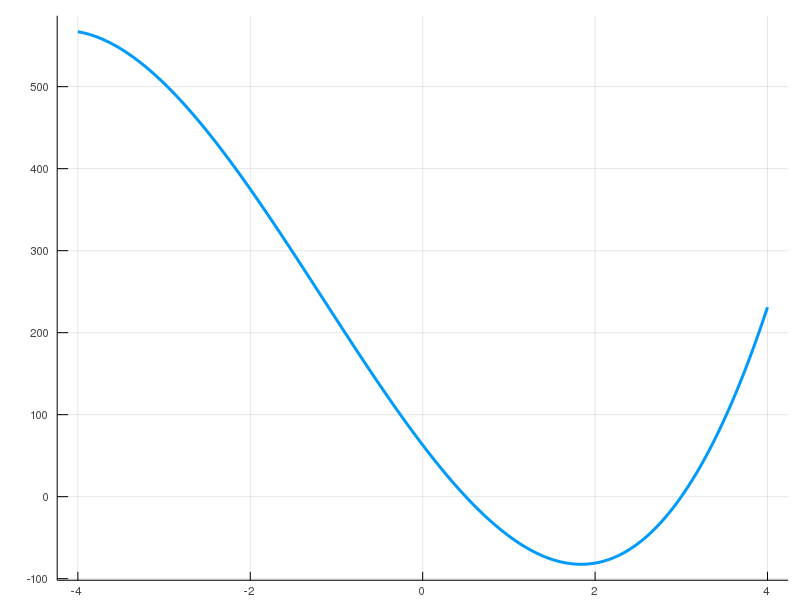
\includegraphics[width=70mm,scale=0.5]{wiel3}
	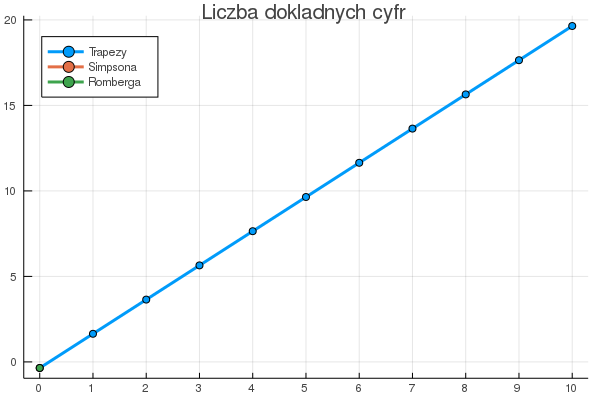
\includegraphics[width=80mm,scale=0.5]{wiel_blad3}
\end{figure}
\begin{remark}
\centering
Wykres funkcji \(f(x) = 6x^3 + 21x^2 - 138x + 63 \) oraz liczba dokładnych cyfr wyników.
\end{remark}
Metoda Simpsona jest dokładna, bo jej rząd wynosi 3. Dokładność metody trapezów rośnie liniowo. Widać, że pierwsza iteracja metody Romberga jest niedokładna, co nie jest niczym dziwnym, bo w pierwszej iteracji jest tożsama z metodą trapezów. W drugiej iteracji jest równa metodzie Simpsona, więc od tego momentu osiąga już pełną dokładność. \\ \\

Trzeci eksperyment przeprowadzono na \(\displaystyle \int_{-6}^{6} (x^4 - 13x^3 - 36x^2 + 268x + 560)\mathop{dx} \)
\begin{figure}[h!]
	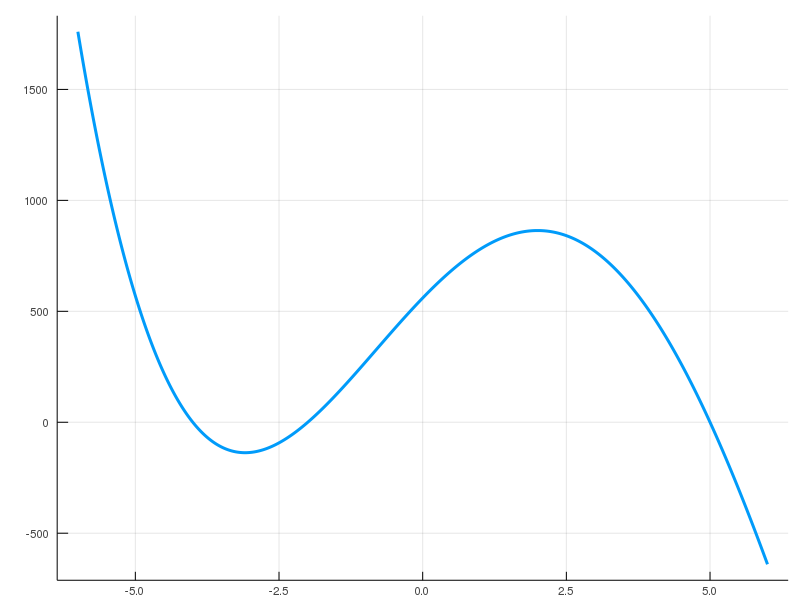
\includegraphics[width=70mm,scale=0.5]{wiel4}
	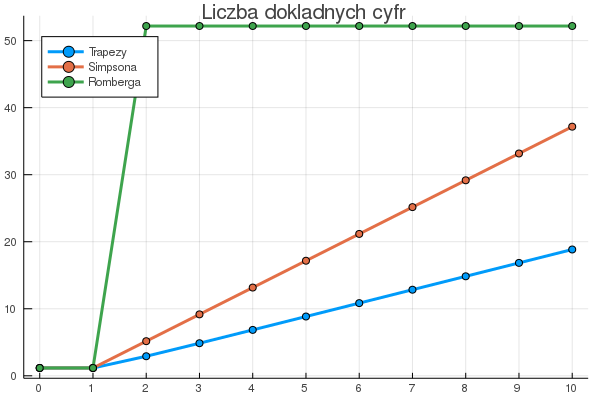
\includegraphics[width=80mm,scale=0.5]{wiel_blad4}
\end{figure}
\begin{remark}
\centering
Wykres funkcji \(f(x) = x^4 - 13x^3 - 36x^2 + 268x + 560 \) oraz liczba dokładnych cyfr wyników.
\end{remark}
Tutaj dokładność metod trapezów i Simpsona rośnie liniowo, z tym że Simpsona rośnie szybciej. Metoda Romberga już dla \(2^2\) przedziałów osiąga dokładność na poziomie ostatnich cyfr mantysy w arytmetyce Float64.
\pagebreak

Czwartemu eksperymentowi poddano wielomian wyższego stopnia niż poprzednie \\ \(\displaystyle \int_{-1}^{1} (3x^{10} - 5x^7 + 2x^6 - 8x^2 - 5)\mathop{dx} \)
\begin{figure}[h!]
	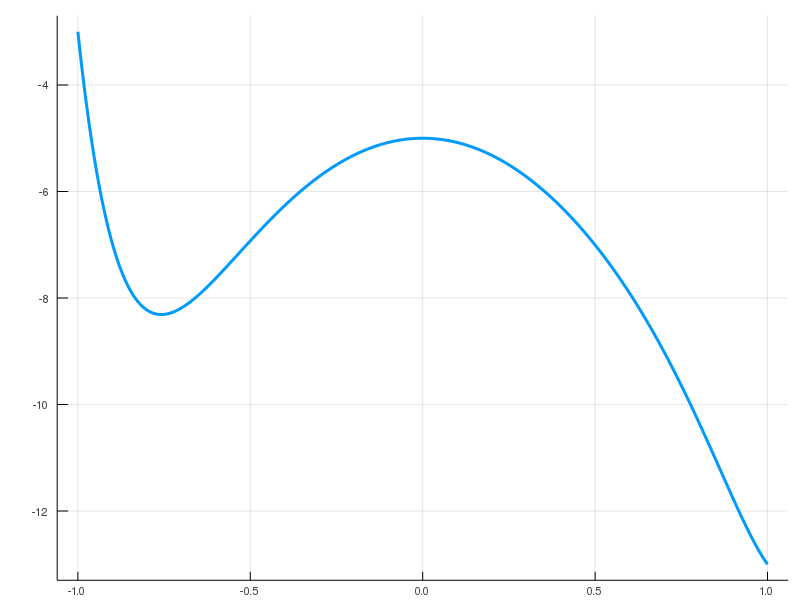
\includegraphics[width=70mm,scale=0.5]{wiel5}
	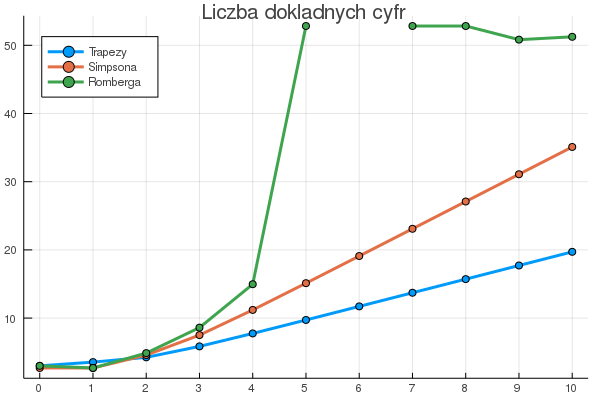
\includegraphics[width=80mm,scale=0.5]{wiel_blad5}
\end{figure}
\begin{remark}
\centering
Wykres funkcji \(f(x) = 3x^{10} - 5x^7 + 2x^6 - 8x^2 - 5 \) oraz liczba dokładnych cyfr wyników.
\end{remark}
Początkowo wszytkie metody mają zbliżoną dokładność, ale dla większej liczby przedziałów, podobnie jak w poprzednim przykładzie, metoda Romberga szybko staje się dokładna, a dokładność metod trapezów i Simpsona rośnie liniowo, ale Simpsona szybciej. \\ \\


Ostatni eksperyment przeprowadzono na wielomianie o symetrycznych względem zera pierwiastkach \(\displaystyle \int_{-4}^{4} \Big((x+5)(x+4)(x+3)(x+2)(x+1)(x-1)(x-2)(x-3)(x-4)(x-5)\Big)\mathop{dx} \)
\begin{figure}[h!]
	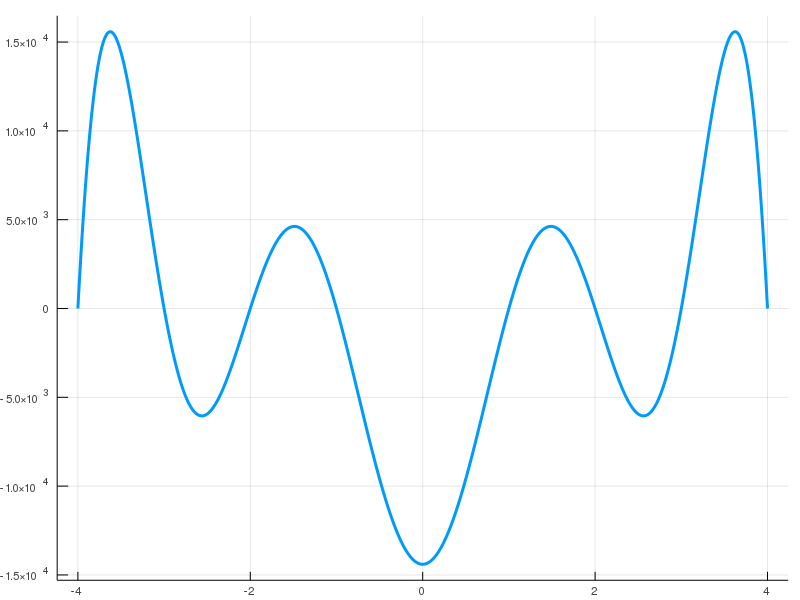
\includegraphics[width=70mm,scale=0.5]{wiel6}
	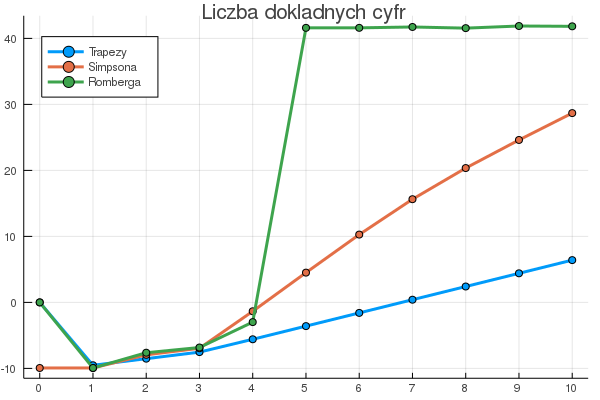
\includegraphics[width=80mm,scale=0.5]{wiel_blad6}
\end{figure}
\begin{remark}
\centering
Wykres funkcji \(f(x) = (x+5)(x+4)(x+3)(x+2)(x+1)(x-1)(x-2)(x-3)(x-4)(x-5) \) \\ oraz liczba dokładnych cyfr wyników.
\end{remark}
Widzimy, że początkow wszystkie metody są bardzo niedokładne. Jednak już dla liczby przedziałów równej \(2^5\) dokładność metody Romberga gwałtownie wzrasta, a później utrzymuje się na tym poziomie. Dokładność metod Simpsona i trapezów rośnie liniowo, ale Simpsona ponownie szybciej.

\subsection{Całka z funkcji wymiernej}
Pierwszy eksperyment został wykonany na funkcji Rungego \(\displaystyle \int_{-1}^{1} \left(\frac{1}{1+25x^2}\right)\mathop{dx} \)
\begin{figure}[h!]
	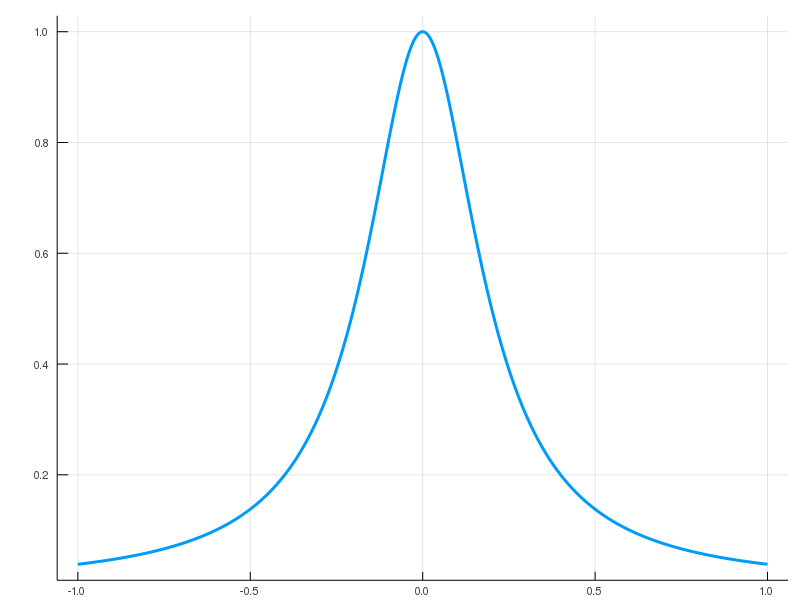
\includegraphics[width=70mm,scale=0.5]{wym1}
	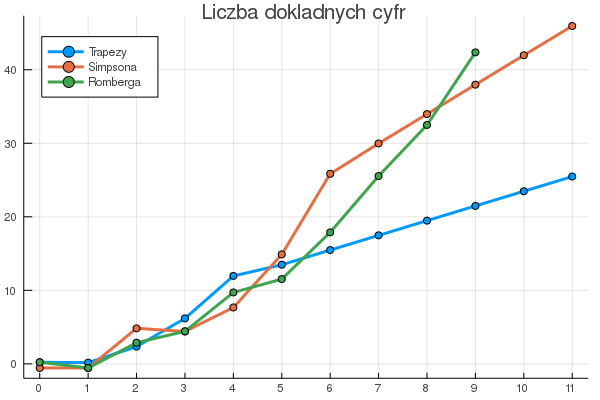
\includegraphics[width=80mm,scale=0.5]{wym_blad1}
\end{figure}
\begin{remark}
\centering
Wykres funkcji \(\displaystyle f(x) = \frac{1}{1+25x^2} \) oraz liczba dokładnych cyfr wyników.
\end{remark}
Można zauważyć, że w powyższym przykładzie metoda Simpsona ma dla pewnych liczb przedziałów lepszą dokładność niż metoda Romberga, czego nie zaobserowaliśmy w przypadku całkowania wielomianów. Jednak znowu metoda Romberga szybciej osiąga maksymalną dokładność niż pozostałe metody. Metoda trapezów znów ma najmniejszą dokładność. \\ \\

Drugi eksperyment został przeprowadzony na funkcji \(\displaystyle \int_{-2}^{2} \left(\frac{x^3 - 6x^2 + 8x - 1}{1+25x^2}\right)\mathop{dx} \)
\begin{figure}[h!]
	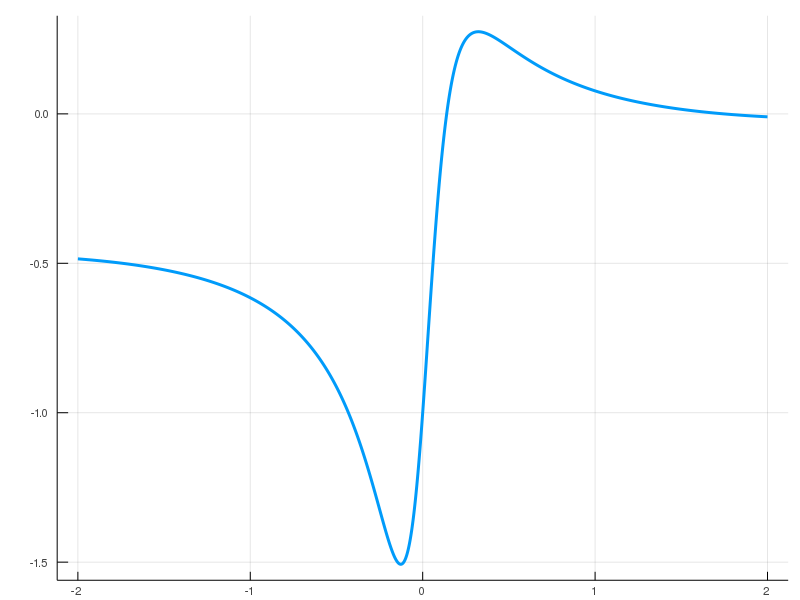
\includegraphics[width=70mm,scale=0.5]{wym2}
	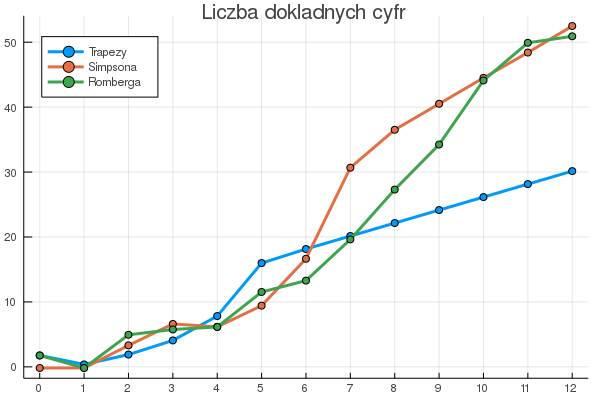
\includegraphics[width=80mm,scale=0.5]{wym_blad2}
\end{figure}
\begin{remark}
\centering
Wykres funkcji \(\displaystyle f(x) = \frac{x^3 - 6x^2 + 8x - 1}{1+25x^2} \) oraz liczba dokładnych cyfr wyników.
\end{remark}
W tym przykładzie możemy zaobserwować, że metody Simpsona i Romberga osiągają niemal maksymalną dokładność dla takiej samej liczby przedziałów.
\pagebreak

Trzeci eksperyment został przeprowadzony na \(\displaystyle \int_{-2}^{2} \left(\frac{x^6 - 6x^5 + 8x - 1}{2x^3 - 7x^2 + 5x - 4}\right)\mathop{dx} \)
\begin{figure}[h!]
	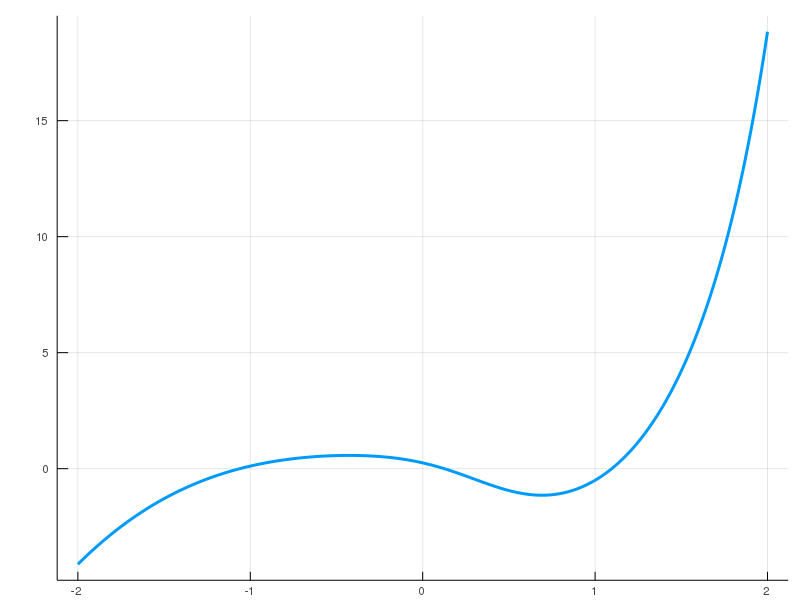
\includegraphics[width=70mm,scale=0.5]{wym3}
	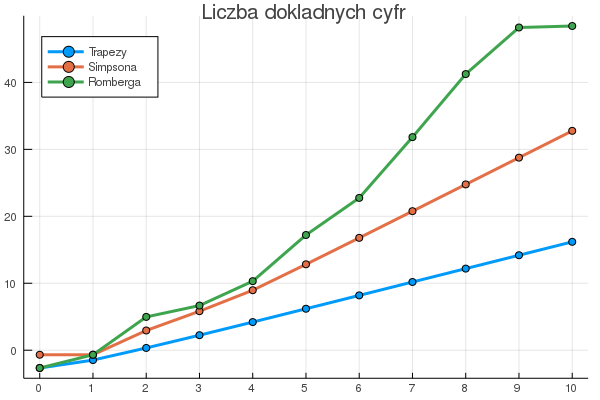
\includegraphics[width=80mm,scale=0.5]{wym_blad3}
\end{figure}
\begin{remark}
\centering
Wykres funkcji \(\displaystyle f(x) = \frac{x^6 - 6x^5 + 8x - 1}{2x^3 - 7x^2 + 5x - 4} \) oraz liczba dokładnych cyfr wyników.
\end{remark}
Dla powyższej funkcji największy przyrost dokładności uzyskuje metoda Romberga, następnie Simpsona, a na końcu trapezów. \\ \\

Ostatni test na funkcjach wymiernych został wykonany na \\ \(\displaystyle \int_{-10}^{10} \left(\frac{x^6 + 6x^5 + 17x^4 + 28x^3 + 29x^2 + 18x + 6}{x^6 + 7x^5 + 26x^4 + 58x^3 + 85x^2 + 75x + 36}\right)\mathop{dx} \)
\begin{figure}[h!]
	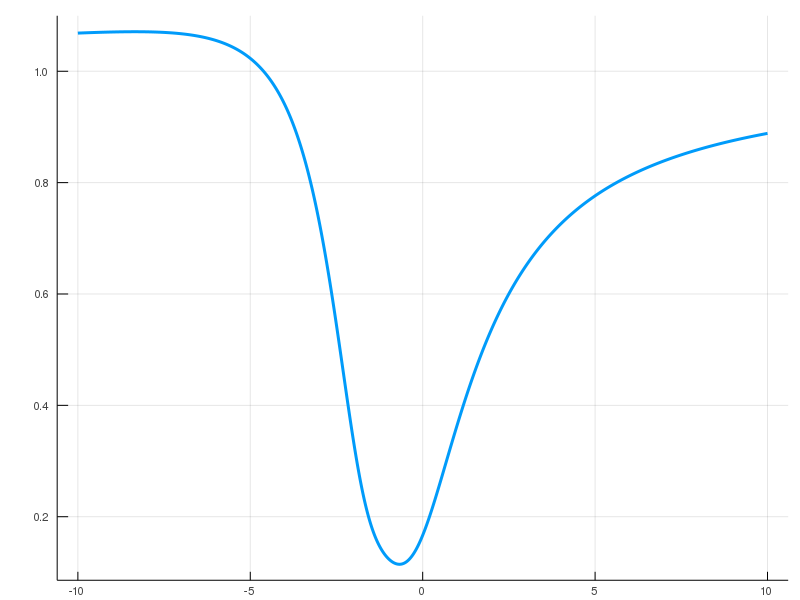
\includegraphics[width=70mm,scale=0.5]{wym4}
	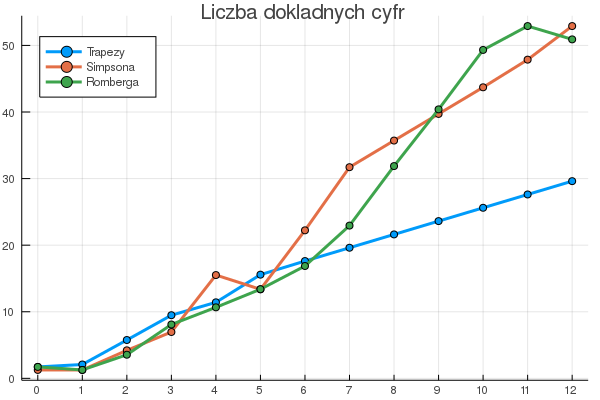
\includegraphics[width=80mm,scale=0.5]{wym_blad4}
\end{figure}
\begin{remark}
\centering
Wykres funkcji \(\displaystyle f(x) = \frac{x^6 + 6x^5 + 17x^4 + 28x^3 + 29x^2 + 18x + 6}{x^6 + 7x^5 + 26x^4 + 58x^3 + 85x^2 + 75x + 36} \) oraz liczba dokładnych cyfr wyników.
\end{remark}
W tym przykładzie, metoda Romberga i Simpsona mają podobny przyrost dokładności, metoda trapezów wypada zdecydowanie gorzej. \\

Wspólnie dla wszystkich testów funkcji wymiernych można zauważyć, że metoda Romberga jest zwykle najoptymalniejsza, jeśli chodzi o wyznaczanie wyniku przy maksymalnej dokładności, chociaż metoda Simpsona może dla szczególnych funkcji dać porównywalną zbieżność, a dla pewnych liczb przedziałów mieć nawet lepszą dokładność niż metoda Romberga. Metoda trapezów w każdym przykładzie wypada najgorzej. Można też dostrzec, że osiągnięcie dobrej dokładności wyników dla całkowania funkcji wymiernej wymaga podzielenia przedziału całkowania na znacznie więcej podprzedziałów niż w przypadku wielomianów.

\subsection{Całka z funkcji wymiernej zmiennych sin(x), cos(x)}
Pierwszy eksperyment został przeprowadzony na \(\displaystyle \int_{-10}^{10} (\sin^2(x) + \cos^3(x) \cdot \sin(x))\mathop{dx} \)
\begin{figure}[h!]
	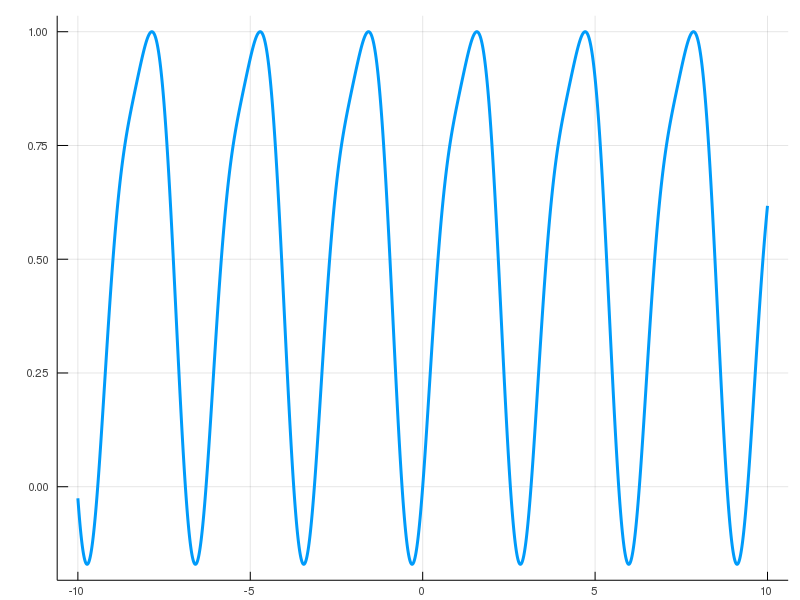
\includegraphics[width=70mm,scale=0.5]{tryg1}
	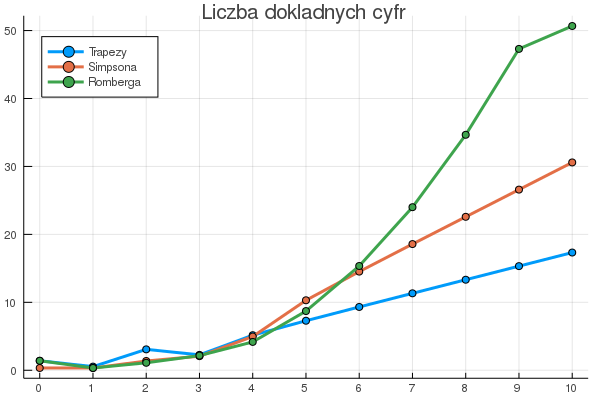
\includegraphics[width=80mm,scale=0.5]{tryg_blad1}
\end{figure}
\begin{remark}
\centering
Wykres funkcji \(\displaystyle f(x) = \sin^2(x) + \cos^3(x) \cdot \sin(x) \) oraz liczba dokładnych cyfr wyników.
\end{remark}


Drugi eksperyment \(\displaystyle \int_{-10}^{10} (\sin(x) + \cos^3(x) \cdot \sin(x) - \sin^2(x) \cdot cos^2(x))\mathop{dx} \)
\begin{figure}[h!]
	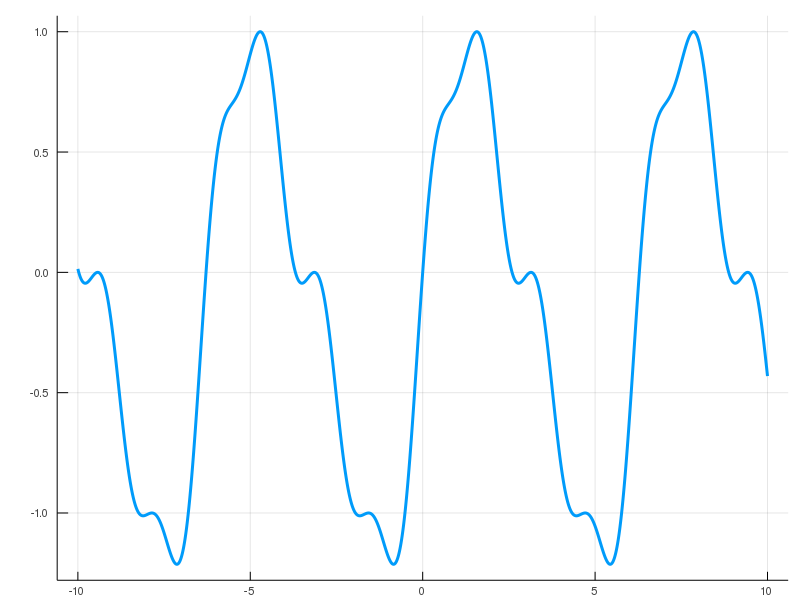
\includegraphics[width=70mm,scale=0.5]{tryg2}
	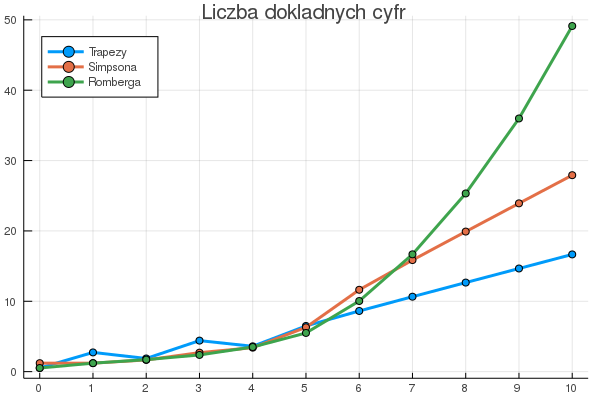
\includegraphics[width=80mm,scale=0.5]{tryg_blad2}
\end{figure}
\begin{remark}
\centering
Wykres funkcji \(\displaystyle f(x) = \sin(x) + \cos^3(x) \cdot \sin(x) - \sin^2(x) \cdot cos^2(x)\) oraz liczba dokładnych cyfr wyników. 
\end{remark}
\pagebreak


Trzeci eksperyment \(\displaystyle \int_{-10}^{10} \left(\frac{\sin(x) + \cos^3(x) \cdot \sin(x) - \sin^2(x) \cdot cos^2(x)}{\sin^2(x) + \cos^3(x) \cdot \sin(x)+1.5}\right)\mathop{dx} \)
\begin{figure}[h!]
	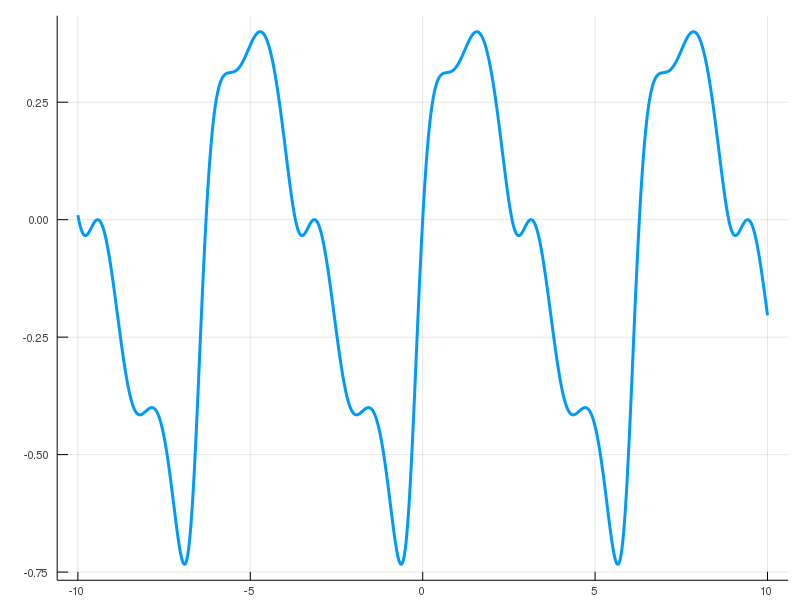
\includegraphics[width=70mm,scale=0.5]{tryg3}
	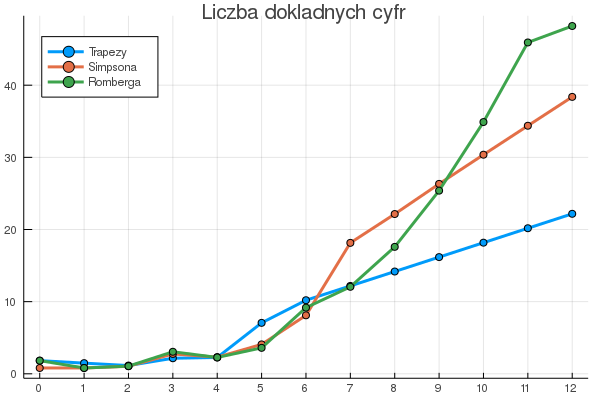
\includegraphics[width=80mm,scale=0.5]{tryg_blad3}
\end{figure}
\begin{remark}
\centering
Wykres funkcji \(\displaystyle f(x) = \frac{\sin(x) + \cos^3(x) \cdot \sin(x) - \sin^2(x) \cdot cos^2(x)}{\sin^2(x) + \cos^3(x) \cdot \sin(x)+1.5}\) oraz liczba dokładnych cyfr wyników.
\end{remark}


Czwarty eksperyment \(\displaystyle \int_{-10}^{10} \left(\frac{\cos(x) - \cos^3(x) \cdot \sin^2(x) - \sin^2(x)}{\sin(x) + \cos(x)\cdot \sin^4(x) - 2 \sin^2(x) \cdot \cos^2(x) + 2}\right)\mathop{dx} \)
\begin{figure}[h!]
	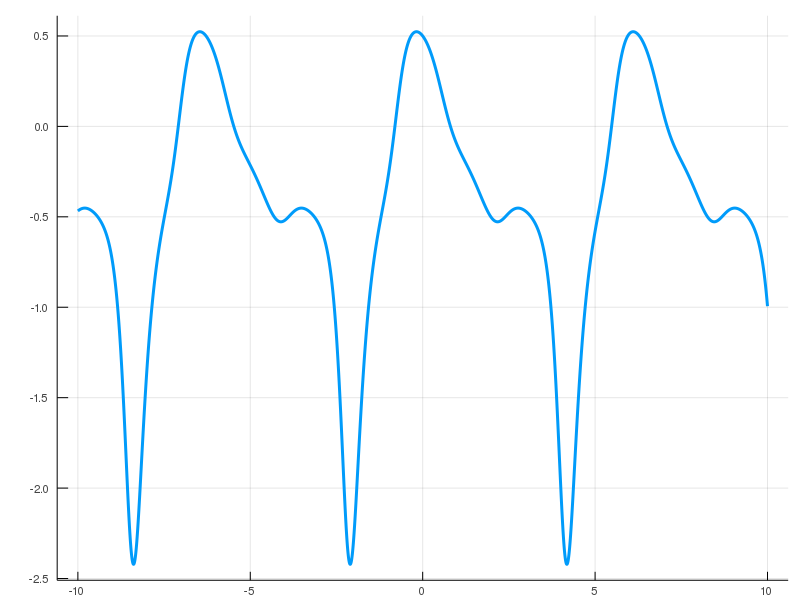
\includegraphics[width=70mm,scale=0.5]{tryg4}
	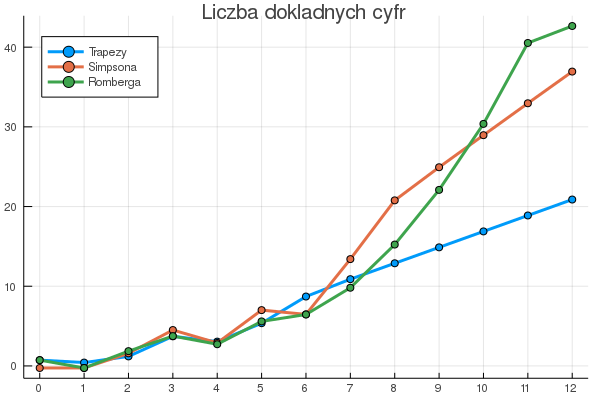
\includegraphics[width=80mm,scale=0.5]{tryg_blad4}
\end{figure}
\begin{remark}
\centering
Wykres funkcji \(\displaystyle f(x) = \frac{\cos(x) - \cos^3(x) \cdot \sin^2(x) - \sin^2(x)}{\sin(x) + \cos(x)\cdot \sin^4(x) - 2 \sin^2(x) \cdot \cos^2(x) + 2}\) oraz liczba dokładnych cyfr wyników.
\end{remark}


W eksperymentach z funkcji wymiernej zmiennych sin(x), cos(x) można zaobserwować, że największą dokładność najszybciej osiąga metoda Romberga, chociaż dla szczególnych przykładów i liczb przedziałów metoda Simpsona może osiągać nawet lepszą dokładność. Metoda trapezów sprawdza się znacznie gorzej.
\pagebreak

\section{Podsumowanie}
Metody trapezów, Simpsona i Romberga są prostymi metodami całkowania numerycznego. Mimo to pokazane zostało, że przy ich użyciu można z dosyć dobrze przybliżać całki z wielomianów, funkcji wymiernych i funkcji wymiernych zmiennych sin(x), cos(x). Złożona metoda trapezów wymaga względnie dużo większej liczby przedziałów do dobrego przybliżenia całki niż metoda Romberga. Metoda Simpsona okazuje się działać lepiej niż metoda trapezów, chociaż wciąż dla zdecydowanej większości przykładów wydaje się znacząco gorsza od metody Romberga. Widać więc, że zwiększanie stopnia wielomianu, którym na przedziałach przybliżana jest badana funkcja, niekoniecznie jest najlepszym pomysłem. Szczególnie, że dla odpowiednio gładkiej, regularnej funkcji i dla bardzo małego przedziału można powiedzieć, że jest na nim prawie liniowa, więc przybliżanie jej na takim przedziale wielomianem wysokiego stopnia może okazać się zbyteczne. O wiele optymalniejsze może się więc okazać stopniowe polepszanie wyników otrzymanych z najprostszych metod, tak jak w przypadku metody Romberga postępuje się ze złożoną metodą trapezów.

\begin{thebibliography}{10}
\bibitem{Kincaid} David Kincaid, Ward Cheneym, przekład i redakcja Stefan Paszkowski,
\emph{Analiza numeryczna},
Wydawnictwo Naukowo-Techniczne, Warszawa, 2006.

\bibitem{Chwiej} Tomasz Chwiej,
\emph{Całkowanie numeryczne przy użyciu kwadratur},
Akademia Górniczo-Hutnicza, 2015, \url{http://home.agh.edu.pl/~chwiej/mn/calkowanie_2015.pdf}

\bibitem{Cruz} D. Cruz-Uribe, C.J. Neugebauer,
\emph{Sharp error bounds for the trapezoidal rule and Simpson's rule},
2002, \url{http://www.emis.de/journals/JIPAM/images/031_02_JIPAM/031_02.pdf}

\bibitem{Mysovskikh} Romberg method. I.P. Mysovskikh (originator),
\emph{Encyclopedia of Mathematics},
\url{http://www.encyclopediaofmath.org/index.php?title=Romberg_method&oldid=16161}

\end{thebibliography}

\end{document}